\documentclass[bachelor, och, labwork]{shiza}

\usepackage{subfigure}
\usepackage{tikz,pgfplots}
\pgfplotsset{compat=1.5}
\usepackage{float}

\usepackage{titlesec}
\setcounter{secnumdepth}{4}
\titleformat{\paragraph}
{\normalfont\normalsize}{\theparagraph}{1em}{}
\titlespacing*{\paragraph}
{35.5pt}{3.25ex plus 1ex minus .2ex}{1.5ex plus .2ex}

\titleformat{\paragraph}[block]
{\hspace{1.25cm}\normalfont}
{\theparagraph}{1ex}{}
\titlespacing{\paragraph}
{0cm}{2ex plus 1ex minus .2ex}{.4ex plus.2ex}

% --------------------------------------------------------------------------%


\usepackage[T2A]{fontenc}
\usepackage[utf8]{inputenc}
\usepackage{graphicx}
\graphicspath{ {./images/} }
\usepackage{tempora}

\usepackage[sort,compress]{cite}
\usepackage{amsmath}
\usepackage{amssymb}
\usepackage{amsthm}
\usepackage{fancyvrb}
\usepackage{listings}
\usepackage{listingsutf8}
\usepackage{longtable}
\usepackage{array}
\usepackage[english,russian]{babel}

\usepackage[colorlinks=true]{hyperref}
\usepackage{url}

\usepackage{underscore}
\usepackage{setspace}
\usepackage{indentfirst} 
\usepackage{mathtools}
\usepackage{amsfonts}
\usepackage{enumitem}
\usepackage{tikz}
\usepackage{minted}

\newcommand{\eqdef}{\stackrel {\rm def}{=}}
\newcommand{\specialcell}[2][c]{%
\begin{tabular}[#1]{@{}c@{}}#2\end{tabular}}

\renewcommand\theFancyVerbLine{\small\arabic{FancyVerbLine}}


\begin{document}

% \chair{Кафедра теоретических основ компьютерной безопасности и криптографии}

\title{Рекурсивные алгоритмы. Упр 3.2}

\course{3}

\group{331}

\department{факультета КНиИТ}

\napravlenie{10.05.01 "--- Компьютерная безопасность}

\author{Никитина Арсения Владимировича}

\satitle{доцент}

\saname{А. Н. Гамова}

\date{2022}

\maketitle

%-------------------------------------------------------------------------------
\tableofcontents

\intro
В данной работе будут рассмотрены принципы рекурсивных алгоритмов, в частности
алгоритма получения всех возможных перестановок элементов заданного множества
без использования дополнительной памяти.

\section{Постановка задачи}
Напишите процедуру формирования на том же месте всех $n!$ перестановок для $n$
элементов $a_1,...,a_n$, то есть без дополнительного массива. После формирования
очередной перестановки можно, например, обратиться к процедуре $Q$ (с параметром),
которая напечатает полученную перестановку.

Указание: задачу формирования всех перестановок элементов $a_1,...,a_m$ можно
считать состоящей из $m$ подзадач формирования всех перестановок для элементов
$a_1,...,a_{m-1}$, за которыми следует $a_m$. Причем в $i$-й подзадаче вначале
меняются местами элементы $a_1 ~\text{и}~ a_m$

\section{Рекурсивный объект}

\textit{Рекурсивным} называется объект, частично состоящий или определяемый с
помощью самого себя.

Мощность рекурсивного определения заключается в том, что оно позволяет с помощью
конечного высказывания определить бесконечное вычисление, причем программа не 
будет содержать явных повторений. Однако рекурсивные алгоритмы лучше всего
использовать, если в решаемой задаче, вычисляемой функции или структуре
обрабатываемых данных рекурсия уже присутствует явно. В общем виде рекурсивную
программу $P$ можно выразить как некоторую композицию $P$ из множества
операторов $S$ (не содержащих $P$) и самой $P$:
\begin{center}$P=P[S,P]$\end{center}

Для выражения рекурсивных программ необходимо и достаточно иметь понятие
процедуры или подпрограммы, поскольку они позволяют дать любому оператору имя,
с помощью которого к нему можно обращаться. Если некоторая процедура $P$
содержит явную ссылку на саму себя, то ее называют \textit{прямо рекурсивной}.
Если же $P$ ссылается на другую процедуру $Q$, содержащую (прямую или косвенную)
ссылку на $P$, то $P$ называют \textit{косвенно рекурсивной}.

Подобно операторам цикла, рекурсивные процедуры могут приводить к
не заканчивающимся вычислениям, и, поэтому на эту проблему следует особо обратить
внимание. Очевидно основное требование, чтобы рекурсивное обращение к $P$
управлялось некоторым условием $B$, которое в какой-то момент становится ложным.

\section{Описание алгоритма получения всех перестановок множества}
Как и было сказано в указании к реализации алгоритма, для того, чтобы
не было лишних затрат по памяти, можно сразу выводить текущую перестановку
в консоль, что и реализовано с помощью вспомогательной функции $print\_permuration$.
Данная функция получает массив, в котором переставлены некоторые элементы
и выводит в консоль порядковый номер текущей перестановки (благодаря глобальной
переменной $current$), а также саму перестановку $current\_permutation$.
Данную функцию требуется вызвать до вызова основной рекурсивной функции 
$next\_permutation$ для того, чтобы вывести в консоль самую первую перестановку.

Самая первая перестановка получается путем сортировки входного множества.

Затем происходит единственный вызов из основной части программы рекурсивной
функции $next\_set$ от отсортированного множества и от его размера.

Абсолютно все перестановки получаются в лексикографическом порядке.

Итак, алгоритм получения всех перестановок выглядит следующим образом:

\begin{enumerate}
    
\item Необходимо просмотреть текущую перестановку справа налево и при этом 
следить за тем, чтобы каждый следующий элемент перестановки (элемент с большим 
номером) был не более чем предыдущий (элемент с меньшим номером). Как только данное 
соотношение будет нарушено необходимо остановиться и отметить текущее число 
(позиция 2).

\item Снова просмотреть пройденный путь справа налево пока не дойдем до первого 
числа, которое больше чем отмеченное на предыдущем шаге. 

\item Затем нужно поменять местами два полученных элемента.

\item Теперь в части массива, которая размещена справа от позиции $1$ надо 
отсортировать все числа в порядке возрастания. 

\item Поскольку до этого они все были уже записаны в порядке убывания 
необходимо эту часть подпоследовательность просто перевернуть.

\item Затем происходит вызов процедуры печати в консоль полученной перестановки с
увеличением глобальной переменной $current$ на единицу.

\item Затем рекурсивный вызов функции получения следующей перестановки.

\end{enumerate}

\section{Результаты тестирования программы}

        \begin{figure}[H]
            \centering
            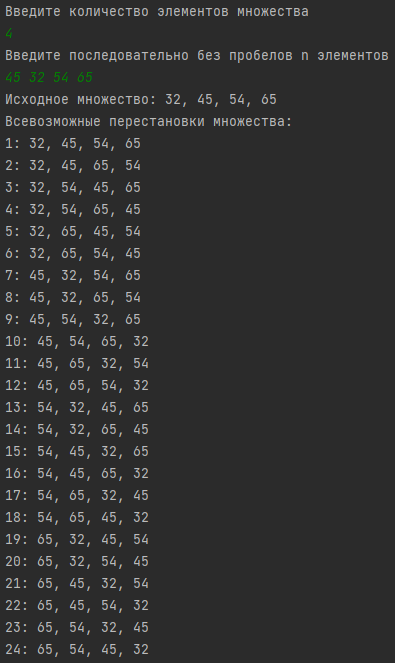
\includegraphics[width=0.8\textwidth]{1.png}
            \caption{}
        \end{figure}

\section{Программная реализация алгоритма}

\inputminted[linenos,breaklines=true, fontsize=\small, style=bw]{python}{1.py}

\section{Оценка работы алгоритма}

Для исследования производительности рассмотренного алгоритма рассмотрим его
составляющие.

Так как рекурсивная функция получения перестановок получает перестановки в 
лексикографическом порядке, требуется вызвать ее от отсортированного в
возрастающем порядке массива, поэтому изначально выполняется сортировка
массива с помощью встроенной функции $sorted()$, использующей оптимизированный
алгоритм быстрой сортировки. Поэтому данную часть программы можно асимптотически
оценить в $O(n\cdot\log n )$.

Затем происходит печать первой перестановки (исходного множества в
отсортированном по возрастанию порядке), что занимает $O(n)$.

Затем происходит вызов рекурсивной функции $next\_permuration$, асимптотика
которого равна $O(n!)$, но так как внутри нее происходит вызов функции печати
перестановки, асимптотика которого равна $O(n)$, то в итоге общая асимптотика
равна $O(n \cdot n!)$.


Получаем общую асимптотику получения всех перестановок: 
\begin{center}
    $O((n \cdot n! + n \cdot \log n) = O(n^2 \cdot (n-1)!)$
\end{center} 


\conclusion

Итак, в данной работе был рассмотрен алгоритм получения всех $n!$ перестановок
множества и вывода их в консоль без использования дополнительной памяти c
помощью прямо рекурсивной функции. Произведена оценка его работы. Асимптотика 
работы данного алгоритма составляет $O(n \cdot n!)$. 

\end{document}